\documentclass[11pt, a4paper]{article}

\usepackage{a4wide}
\usepackage{amsmath,amssymb,amsthm,amscd}
\usepackage{natbib}
\usepackage[pdftex]{graphicx}
\usepackage[affil-it]{authblk}
\usepackage{sidecap}
\usepackage[font=small,labelfont=bf]{caption}


%\usepackage{showkeys}

\usepackage[all]{xy}

\newcommand{\bb}[1]{\begin{equation}\label{#1}}
\newcommand{\ee}{\end{equation}}
\newcommand{\vc}[1]{{\bf #1 }}
\renewcommand{\vec}[1]{{\bf #1}}
\newcommand{\Sum}[1]{\sum\limits_{#1}}
\newcommand{\Int}[1]{\int\limits_{#1}}
\newcommand{\Prod}[1]{\prod\limits_{#1}}
\newcommand{\const}{\operatorname{const}}
\newcommand{\ul}{\underline}
\newcommand{\ol}{\overline}
\newcommand{\tr}{\operatorname{tr}}
\newcommand{\bbA}{\mathbb A}
\newcommand{\bbR}{\mathbb R}
\newcommand{\bbN}{\mathbb N}
\newcommand{\bbZ}{\mathbb Z}
\newcommand{\bbC}{\mathbb C}
\newcommand{\bbT}{\mathbb T}
\newcommand{\QB}{\mathcal H}
\newcommand{\PQB}{\tilde{\mathcal H}}
\newcommand{\CQB}{\mathcal H'}
\newcommand{\Ad}{\operatorname{Ad}}
\newcommand{\ad}{\operatorname{ad}}
\newcommand{\gh}{\operatorname{gh}}
\newcommand{\Der}{\operatorname{Der}}
\newcommand{\Aut}{\operatorname{Aut}}
\newcommand{\aut}{\operatorname{aut}}
\newcommand{\Diff}{\operatorname{Diff}}
\renewcommand{\dim}{\operatorname{dim}}
\newcommand{\Vol}{\operatorname{Vol}}
\newcommand{\Pf}{\operatorname{Pf}}
\newcommand{\Cov}{\operatorname{Cov}}

\newcommand{\g}{{\bf g}}
\newcommand{\h}{{\bf h}}
\renewcommand{\d}{{\bf d}}
\newcommand{\e}{{\bf e}}
\renewcommand{\t}{{\bf t}}
\newcommand{\lpartial}{\overset{\rightarrow}{\partial}}
\newcommand{\rpartial}{\overset{\leftarrow}{\partial}}
\newcommand{\lder}[1]{\overset{\rightarrow}{\vc #1}}
\newcommand{\rder}[1]{\overset{\leftarrow}{\vc #1}}
\newcommand{\supp}{\operatorname{supp}}
\newcommand{\im}{\operatorname{Im}}
\renewcommand{\ker}{\operatorname{Ker}}
\newcommand{\Var}{\operatorname{Var}}


%define the \identy operator
\def\litID{{\sf id}}
\def\identy{{\mathsurround0pt\mathchoice{\textidenty}{\textidenty}{\scptidenty}{\scptidenty}}}
\def\scptidenty{\setbox0\hbox{$\scriptstyle1$}\bothidenty}
\def\textidenty{\setbox0\hbox{$1$}\bothidenty}
\def\bothidenty{\rlap{\hbox to.97\wd0{\hss\vrule height.06\ht0 width.82\wd0}}
 \copy0\rlap{\kern-.36\wd0\vrule height1.05\ht0 width.05\ht0}\kern.14\wd0}
%end of definition \identy

\newcommand{\bbM}{\mathbb M}
\newcommand{\bt}{\pmb\theta}
\newcommand{\Bt}{\pmb\Theta}
\newcommand{\dt}{\mathit{dt}}
\newcommand{\eq}{\text{eq}}




\begin{document}
\title{Parameter Inference for a Simple Stochastic Hydrological Model}

\author{C. Albert\thanks{\noindent Email: carlo.albert@eawag.ch} \,,
S. Ulzega \,, P. Reichert}
\affil{Eawag, Swiss Federal Institute of Aquatic Science and Technology, 8600 D\"ubendorf, Switzerland}
\maketitle

In this paper, we study the feasibility of a full Bayesian inference, for simple conceptual rainfall-runoff models with scale-invariant noise.
We start with a single linear reservoir and describe the dynamics of its water content, $S(t)$, by means of the stochastic differential equation
\begin{equation}\label{sde}
\dot{S}(t) = r(t) - \frac{1}{K}\left(1+\frac{\gamma}{2}\right) S(t)
+
\sqrt{\frac{\gamma}{K}} S(t){\eta}(t)\,,
\end{equation}
where $r(t)$ describes the rain input and $\eta(t)$ denotes white noise, i.e.,
\begin{equation}\label{whitenoise}
\langle\eta(t)\eta(t')\rangle = \delta(t-t')\,.
\end{equation}
Given rainfall and runoff time-series, we want to infer the two system parameters $K$ and $\gamma$, measuring, respectively, the {\em retention time}, and the noise.
The noise parameter is dimensionless, which renders the noise term scale-invariant.
Due to the state-dependence of the noise term, eq. (\ref{sde}) is ill-defined unless we specify the discretization convention.
For computational reasons, we work with the {\em Stratonovich} convention.
Our parametrization is such that, for constant rain input $r(t)=r$, the mean of $S$ converges to $Kr$, in the long-time limit (see below).

According to \cite{lau_2007_StateDepDiff}, the probability $P(S)$ of finding the system in a state $S$ at time $t = T$ given that it was in an initial state $S_0$ at time $t = 0$, can be expressed in the form of a path integral as,

\begin{equation}\label{pathint}
P(S) = \int_{S_0}^{S} e^{-\tilde{\mathcal S}[\dot{S}(t),S(t)]} \mathcal{D}S \,,
\end{equation}
where the integral extends over all paths starting at $S_0$ and ending at $S$.
The path-measure $\mathcal DS$ is the formal limit $\Delta t\rightarrow 0$ of the discretized measure
\begin{equation}\label{pathmeasure}
{\mathcal D}S
=
\prod_{i}
\frac{dS_i}{\sqrt{2\pi \mathit{\Delta t} \gamma/K }S_i}\,.
\end{equation}
The {\em action} is a functional defined on paths $\tilde{\mathcal S}:[0,T]\longrightarrow \mathbb R_+$ and reads as
\begin{equation}\label{action}
  \tilde{\mathcal S}[\dot{S}(t),S(t)]
  =
  \int_0^T
  dt
  \left\{
    \frac{K}{2\gamma S^2(t)}
    \left(
        \dot S(t)
        -
        r(t)
        +
        \frac{1+\gamma}{K}S(t)
    \right)^2
    -
    \frac{2+\gamma}{4K}
  \right\}
 \,.
\end{equation}
Note that the action includes the Jacobian that arises when changing coordinates from ${\eta(t)}$ to $S(t)$ and ensures the normalization condition $\int{ P(S) \mathit{dS}}=1$.

It is possible to calculate the equilibrium distribution $P_{\text{eq}}(S) = \lim_{T\rightarrow\infty} P(S(T))$ in the simple case of a constant rain input $r_{0}$. Systems at thermal equilibrium must fulfill detailed balance, i.e.,
\begin{equation}\label{detailed_balance}
P(S_1 t_1 | S_0 t_0 ) P_{\text{eq}}(S_0) = P(S_0 t_1 | S_1 t_0 ) P_{\text{eq}}(S_1) \,,
\end{equation}
where $P(S_1 t_1 | S_0 t_0 )$ is the conditional probability for the state $S_1$ at time $t_1$ given the initial state $S_0$ at time $t_0$ and $P(S_0 t_1 | S_1 t_0 )$ is the conditional probability for the reverse path $\overline{S}(t) = S(-t)$. Assuming a solution in the form

\begin{equation}\label{Peq}
  P_{\text{eq}}(S)
  \propto
  e^{-\mathcal{H}(S)}\,,
\end{equation}

equation (\ref{detailed_balance}) can be rewritten as

\begin{equation}\label{detailed_balance_2}
P(S_1 t_1 | S_0 t_0 ) = P(S_0 t_1 | S_1 t_0 ) \exp^{-\int_{t_0}^{t_1} dt \frac{dS}{dt}\frac{\mathcal{H}}{S}}\,.
\end{equation}

After plugging in (\ref{pathint}) for the conditional probabilities, and using the action (\ref{action}), equation (\ref{detailed_balance_2}) yields

\begin{equation}\label{constant_rain_H}
-r_{0}+\frac{1+\gamma}{K}S
=
\frac{\gamma S^2}{2K}
\frac{d \mathcal{H}(S)}{dS}\,.
\end{equation}

In order to go from (\ref{detailed_balance_2}) to (\ref{constant_rain_H}) we have exploited the property of the Stratonovich convention that the backward path is evaluated at the same points as the forward path. The solution to (\ref{constant_rain_H}) is, up to an additive constant,

\begin{equation}\label{solution_const_rain}
\mathcal{H}(S)=\frac{2 K r_0}{\gamma S}+\frac{2(1+\gamma)}{\gamma}\ln(S)\,.
\end{equation}

%\begin{figure}
%    \centering
%    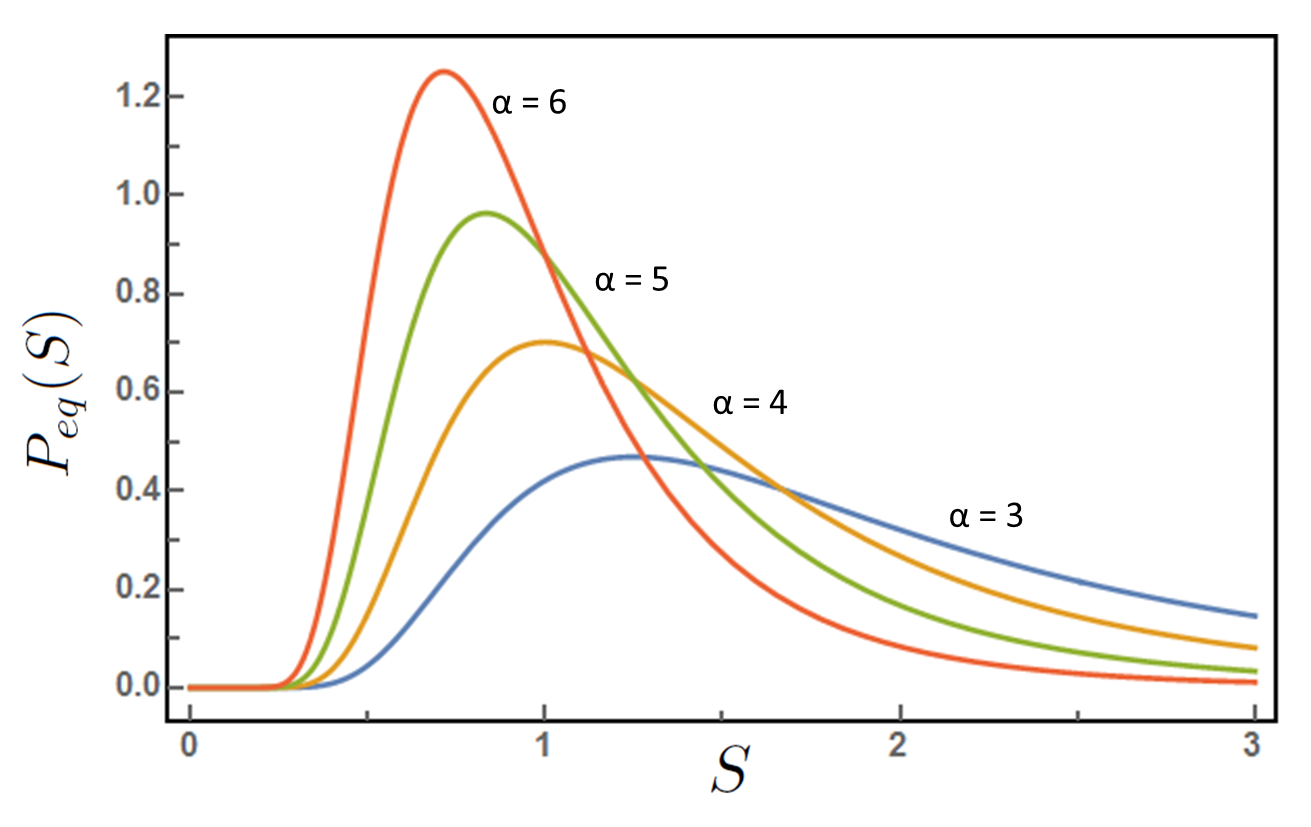
\includegraphics[width=0.6\textwidth]{Figs/InvGamma.png}
%    \caption{Inverse gamma distributions with scale parameter $\beta = 5$ and shape parameters $\alpha = 3,4,5,6$.}
%    \label{fig:inv_gamma}
%\end{figure}

Thus, it turns out that $P_{\text{eq}}(S)$ is described by an inverse gamma distribution, $\Gamma^{-1}(\alpha,\beta)$ with scale parameter $\beta=2Kr_{0}/\gamma$ and shape parameter $\alpha=(2+\gamma)/\gamma$, i.e.,

\begin{equation}\label{inverse_gamma}
  P_{\text{eq}}(S)
  \propto
  S^{-2(1+\gamma)/\gamma}e^{-2Kr_{0}/(\gamma S)}\,,
\end{equation}

whose mean equals the equilibrium solution of the unperturbed system,

\begin{equation}
  \langle S\rangle_{\eq}=Kr_{0},
\end{equation}

and whose variance, for $\gamma< 2$, is given by

\begin{equation}
  \langle (S - \langle S\rangle_{\eq})^2\rangle_{\eq}
  =
  K^2r_{0}^2
  \frac{\gamma}{2-\gamma}\,.
\end{equation}

Note that the variance diverges for $\gamma\geq 2$.

\vspace{\baselineskip}

Let us consider now the general case of a time dependent rain input $r(t)$ with the following time-series of {\em observed} outputs,

\begin{equation}\label{data}
  y_i=\frac{1}{K}S(t_i)+\sigma\epsilon_i\,,\quad i=1,\dots,n\,,
\end{equation}

where the times $t_i$ are chosen so that $0=t_1<t_2<\dots < t_n=T$ and the $\epsilon_i$ are uncorrelated standard normal random variables.
The {\em likelihood} function for the data (\ref{data}) is, up to a factor that doesn't depend on the model parameters, given by the path-integral

\begin{equation}\label{likelihood}
  f(\vc y | \bt)
  \propto
  \int
  \exp\bigg[
    -{\tilde{\mathcal S}}[\dot{S},S]
    -\frac{1}{2}
    \sum_{i=1}^n
    \frac
    {(y_i-S(t_i)/K)^2}
    {\sigma^2}
  \bigg]
  {\mathcal D} S(\bt)\,,
\end{equation}

with the parameter vector $\bt=(K,\gamma)^T$. Choosing for the parameters $K$ and $\gamma$ the improper prior given by

\begin{equation}\label{prior}
  f(\bt)
  =  f(K) f(\gamma) = \frac{1}{K \gamma} \,,
\end{equation}

{\em parameter inference} means generating a sufficiently large sample of parameter vectors from the posterior
\begin{equation}\label{posterior}
  f(\bt|\vc y)\propto f(\vc y|\bt)f(\bt)\,.
\end{equation}

We replace the variable $S(t)$ and the parameter $K$ by the dimensionless quantities, $q(t)$ and $\beta$, respectively, by means of the transformations
\begin{equation}
  \beta=\sqrt{\frac{T\gamma}{K}}\,,\quad
  S(t)=\frac{T\gamma r(t)}{\beta^2}e^{\beta q(t)}\,.
\end{equation}
In terms of these dimensionless variables and parameters the posterior reads (without prior)
\begin{equation}\label{posterior_pathint}
  f(\bt | \vc y)
  \propto
  \int
  \exp\bigg[
    -{\tilde{\mathcal S}}[\dot{q}(t),q(t)]
    -\frac{1}{2}
    \sum_{i=1}^n
    \frac
    {(y_i-r_ie^{\beta q_i})^2}
    {\sigma^2}
    %-\ln(K\gamma)
  \bigg]
  {\mathcal Dq}
  \,,
\end{equation}
%\prod_{t}
%\frac{dS(t)}{\sqrt{2\pi \mathit{\Delta t} \gamma/K }S(t)}\,,
where $r_i$ and $q_i$ represent $r(t)$ and $q(t)$, respectively, at time $t_i$. In the transformed variables the path-measure takes the form, up to a parameter-independent multiplicative factor,

\begin{equation}\label{pathmeasure_q}
{\mathcal Dq}
=
\prod_{t}
dq(t)\,,
\end{equation}

while the action can be rewritten in the compact form,

\begin{equation}\label{action_new}
\tilde {\mathcal S}[\dot{q},q]
=
\frac{1}{2T}
\int_0^T \dt \left\{\left(
    T\dot q(t)
    +
    \rho(t)
    -
    \frac{\beta}{\gamma}e^{-\beta q(t)}\right)^2
    -
    \frac{(2+\gamma)\beta^2}{2\gamma}
\right\} \,,
\end{equation}

with
\begin{equation}\label{rho}
\rho(t)=\frac{T\dot r(t)}{\beta r(t)}+\frac{\beta(\gamma+1)}{\gamma}
=
\frac{T}{\beta}\frac{d \left[\ln r(t)\right]}{dt}+\frac{\beta(\gamma+1)}{\gamma}\,.
\end{equation}

In order to ease the numerical computations, it is useful to introduce a generalized time-dependent Hamiltonian,

\begin{equation}\label{H}
  \mathcal{H}_q(q,t)
  =
  \frac{1}{\gamma}e^{-\beta q}+q\rho(t)\,,
\end{equation}

and rewrite the action (\ref{action_new}) as,

\begin{multline}\label{action_final}
{\mathcal S}[\dot{q},q]
=
\frac{1}{2T}
\int_0^T dt\left\{
    T^2\dot q^2(t) +
    \left(\rho(t)-\frac{\beta}{\gamma}e^{-\beta q(t)}\right)^2 -
    2T\frac{\partial \mathcal{H}_q(q,t)}{\partial t} -
     \frac{(2+\gamma)\beta^2}{2\gamma}
\right\}
\\
+ \mathcal{H}_q(q(T),T) - \mathcal{H}_q(q(0),0)
\\
= \frac{1}{2T}
\int_0^T dt\left\{
    T^2\dot q^2(t) +
    \left(\rho(t)-\frac{\beta}{\gamma}e^{-\beta q(t)}\right)^2 -
    2Tq(t)\dot\rho(t) -
    \frac{(2+\gamma)\beta^2}{2\gamma}
\right\}
\\
+
    \frac{1}{\gamma}e^{-\beta q(T)}+q(T)\rho(T)
   -\frac{1}{\gamma}e^{-\beta q(0)}-q(0)\rho(0)
\,.
\end{multline}

Since the integral on the r.h.s. of (\ref{posterior_pathint}) is very expensive to calculate, we will sample simultaneously parameter vectors $\bt$ and discretized system realizations $q(t)$ directly from an appropriate discretization of the kernel of (\ref{posterior_pathint}).
Since this distribution is very high dimensional and strongly correlated, we employ the method called {\em Hamiltonian Monte Carlo} (HMC) introduced by \cite{duane_1987_HMC}.
This method interprets the exponent of the kernel of the posterior as the potential of a one-dimensional statistical mechanical system. Each degree of freedom, $q(t)$ and $\bt$ in our case, is paired with a conjugate variable, $p(t)$ and ${\pmb\pi}$, respectively, and the system is defined by the  Hamiltonian

\begin{equation}\label{Hamiltonian}
    \mathcal{H}_{\text{HMC}}(q,\bt; p,{\pmb\pi})
    =
    K( p,{\pmb\pi}) + V( q,\bt)\,,
\end{equation}

where

\begin{equation}\label{K}
   K( p,{\pmb\pi})
   =
   \int \frac{ p^2(t)}{2m_q}dt
   + \sum_{\alpha=1}^s\frac{\pi_\alpha^2}{2m_\alpha}\,,
\end{equation}

where in our case $s=2$, and $V( q,\bt)$ is the logarithm of the kernel of (\ref{posterior_pathint}).
The HMC method, which is a combination of the {\em Metropolis algorithm} by \cite{metropolis_1953_MRT2} and {\em molecular dynamics} methods \textbf{[ref?]}, iterates the following steps

\begin{enumerate}
  \item
  Momenta are sampled from the Gaussian distribution defined by (\ref{K}).
  \item
  A volume-preserving and time-reversible solution to a discretization of Hamilton's equations is calculated numerically (leap-frog algorithm).
  \item
  The discretization error on the energy preservation due to the previous step is corrected by a Metropolis acceptance/rejection step.
\end{enumerate}

The last step is the standard Metropolis algorithm, while the first two steps allow to make relatively large jumps in phase space while maintaining a relatively large acceptance rate.

In particular, step 2 requires the calculation of the gradient of (\ref{Hamiltonian}), which is a somewhat tedious manual labour.
Before we set out to do so, let us first write down the proper discretization of the path-integral (\ref{posterior_pathint}), with the action (\ref{action_final}).
Therefore, let us assume that the measurement time points $\left\{ y_i \right\}_{i=1,\dots, n}$ of the time series (\ref{data}) are equidistantly distributed on the time interval $[0,T]$.
We further partition this interval into $N$ bins, with $N >> 1$, according to the time series $0=t_1<t_2,\dots<t_N=T$, such that the time points $t_{a_{\kappa}}$ with indexes $a_{\kappa} = \kappa (N-1)/n + 1$, where $\kappa = 1,\dots, n$, coincide with the data points $y_i$.
Under these assumptions the discretized versions of $K( p,{\pmb\pi})$ and $V( q,\bt)$ read

\begin{align}
   K( p,{\pmb\pi})
   &=
   \sum_{i=1}^N \frac{ p_i^2}{2m_q}\Delta t
   + \sum_{\alpha=1}^s\frac{\pi_\alpha^2}{2m_\alpha}\,,\label{Kdisc}
   \\
   V(q,\bt)
   &\approx
   \sum_{i=2}^{N}
  \frac{K}{2\gamma\Delta t}
  (q_i-q_{i-1})^2+\sum_{i=2}^{N-1} \frac{\Delta t}{\gamma} \left\{\frac{(\rho_i-e^{-q_i})^2}{2 K}  - q_i \frac{(\rho_i-\rho_{i-1})}{\Delta t} \right\}
  \\
  &- \frac{T (\gamma + 2)}{4 K}+\frac{\left(e^{-q_N}+q_N \rho_{N-1}- e^{-q_1}-q_1 \rho_{1} \right)}{\gamma} \nonumber
  \\
  & + \sum_{\kappa=1}^n \frac{(y_\kappa-r_{a_{\kappa}} e^{q_{a_{\kappa}}})^2}{2\sigma^2} +\ln \left(K^{1-N/2} \gamma^{1+N/2}\right)\nonumber
   \,,\label{Vdisc}
\end{align}

where the last term comes from the path measure (\ref{pathmeasure_q}) and

\begin{equation}\label{rhodisc}
\rho_i = K \frac{\ln(r_{i+1}/r_i)}{\Delta t}+\gamma+1\,.
\end{equation}

%\begin{equation}
%  \dot{q}_i:=\frac{ q_i -  q_{i-1}}{\Delta t}\,,\quad
%  \bar{ q}_i:=\frac{q_i + q_{i-1}}{2}\,,
%\end{equation}
%and the analogous definition of $\dot r_i$ and $\bar r_i$.

For strongly varying rain input or high-frequency output data, $\Delta t$ needs to be chosen small. Thus, the harmonic part of the Hamiltonian becomes stiff and, consequently, the time-step of MD needs to be chosen small, which leads to slow convergence.
To solve this problem, we change coordinates, such that the harmonic part of the Hamiltonian becomes (partly) diagonal and the particle interaction moves to the potential.
One option would be to use the Fourier modes of ${\eta}(t)$ as configurational variables. Calculating the potential requires then an inversion of a Toeplitz matrix. This approach is interesting because, in our case, it allows for an approximate analytical integration of high-frequency modes.

Another approach is the so-called \emph{staging}, described in Tuckerman et al. (1993). This approach is interesting if different time-scales are involved.
We first note that the Hamiltonian $\mathcal{H}_{\text{HMC}}(q,\bt; p,{\pmb\pi})$ (\ref{Hamiltonian}) can be seen as the classical Hamiltonian of a polymer chain with harmonic bonds between neighbouring beads, described by the first harmonic term of $V(q,\bt)$, in an external field described by the other non-harmonic terms of $V(q,\bt)$. Sampling system realizations, each defined by a set of coordinates $\left\{ q_i\right\}$ and parameters $\bt$, is equivalent to sampling states in the polymer dynamics. Thus, let us place $n+1$ equidistant (data) beads on the time domain, the first sitting on $t=0$ and the last on $t=T$. In between, we place $n(j-1)$ equidistant staging beads. So that, in total, we have $nj+1=N$ equidistant beads.

The discretized harmonic part of the action can be rewritten as

\begin{multline}
  \sum_{i=2}^{N}
  \frac{K}{2\gamma\Delta t}
  (q_i-q_{i-1})^2
  \\ =
  \frac{K}{2\gamma}
  \sum_{s=1}^{n}\left\{
    \frac{(q_{(s-1)j+1} - q_{sj+1})^2}{j\Delta t}
    +
    \sum_{k=2}^j
    \frac{k}{(k-1)\Delta t}
    (q_{(s-1)j+k}-q^*_{(s-1)j+k})^2
  \right\}\,,
\end{multline}

with

\begin{equation}
  q^*_{(s-1)j+k}
  =
  \frac{(k-1)q_{(s-1)j+k+1} + q_{(s-1)j+1} }{k}
  \,.
\end{equation}

Following Tuckerman et al. (1993) we apply the coordinate transformation

\begin{equation}
  u_{sj+1} = q_{sj+1}\,,\quad
  u_{sj+k} = q_{sj+k} - q^*_{sj+k}\,,
\end{equation}

with its inverse given by

\begin{equation}
  q_{sj+1} = u_{sj+1}\,,\quad
  q_{sj+k} = \sum_{l=k}^{j+1}\frac{k-1}{l-1}u_{sj+l}
  +\frac{j-k+1}{j}u_{sj+1}\,,
\end{equation}

or equivalently by the recursive relation

\begin{equation}
  q_{sj+k} = u_{sj+k} + \frac{k-1}{k} q_{s+k+1}+ \frac{1}{k}q_{sj+1} \,.
\end{equation}

Moreover, we introduce the following transformation for the parameters,

\begin{equation}\label{params_transform}
\beta = \ln(K/T) \,,\quad \tau=\ln(\gamma)
\end{equation}

and the corresponding transformed vector $\tilde{\bt}=(\beta,\tau)^T$. This transformation ensures that the system parameters $K$ and $\gamma$ will be kept positive during the HMC algorithm.

The potential $V(q,\tilde{\bt})$ can now be split into a fast component that scales linearly or quadratically with $N$ or $n$,

\begin{multline}
  {\mathcal V}_f(\vc u,\tilde{\bt})
  =
  \frac{N e^{\beta-\tau}}{2}
  \sum_{s=1}^n\left\{
    \frac{(u_{(s-1)j+1} - u_{sj+1})^2}{j}
    +
    \sum_{k=2}^j
    \frac{k}{(k-1)}
    u_{(s-1)j+k}^2
  \right\}
  \\
  +
  \frac{N}{2}(\beta-\tau)
      -
    \sum_{s=0}^{n}
    \frac
    {(y_s-r_{sj+1}e^{u_{sj+1}})^2}
    {2 \sigma^2}
  \,,
\end{multline}

where we have used $T = N \Delta t$, and a slow $N-$ and $n-$independent component,

\begin{multline}
{\mathcal V}_s(\vc q,\tilde{\bt})
=
    \sum_{i=2}^{N-1}
        \left\{
            \frac{e^{-(\beta+\tau)}}{2N}
            (\rho_i-e^{-q_i})^2 - e^{-\tau}
            q_i (\rho_i-\rho_{i-1})
        \right\}-\frac{(2+e^\tau)e^{-\beta}}{4}
        \\
    + e^{-\tau} \left( e^{-q_N} + q_N\rho_{N-1}
    - e^{-q_1} - q_1\rho_1\right)
\,.
\end{multline}

In the expressions above we have included the Jacobian associated with (\ref{params_transform}).

\vspace{\baselineskip}

We can now fully exploit the two different time-scales that are involved in the problem. First, the harmonic part of the fast component ${\mathcal V}_f[\dot{\vc u},\vc u]$ can be seen as describing the dynamics of heavy coupled \emph{boundary} data-point beads and lighter uncoupled \emph{staging} beads. The different weights of boundary and staging beads are defined by adjusting their \emph{effective masses}, $m_{\text{bdy}}$ and $m_{\text{st}}$, respectively. These values are used in (\ref{Kdisc}) for the masses $m_{q}$.
Second, the two different ranges of the forces associated with ${\mathcal V}_f(\vc u,\tilde{\bt})$ and ${\mathcal V}_s(\vc q,\tilde{\bt})$ can be efficiently taken into account by applying a reversible reference system propagator algorithm (RESPA), as outlined in Tuckerman et al. (1992). The RESPA algorithm, based on appropriate reversible molecular dynamics integrators, can significantly accelerate simulations of systems that are simultaneously subject to short- and long-range forces by separating the two different time-scales.

The basic idea of the RESPA algorithm is to apply a Trotter decomposition to the system Liouville propagator $\mathcal{L}$ to generate a discrete time propagator factorized into fast and slow contributions. Indeed, as shown in Tuckerman et al. (1992), the propagator $\exp[i \mathcal{L} \Delta \tau ]$ can be written as

\begin{equation}\label{G}
  \mathcal{G}(\Delta \tau)=\exp\left\{ \frac{\Delta \tau}{2} F_s(x) \frac{\partial}{\partial p} \right\} \exp\left\{ i \mathcal{L}_f \Delta \tau  \right\} \exp\left\{ \frac{\Delta \tau}{2} F_s(x) \frac{\partial}{\partial p} \right\}\,,
\end{equation}

where for the sake of clarity we have assumed a one-dimensional system. The argument can be easily extended to our multi-dimensional case. In (\ref{G}) $F_s$ is the force associated with the slowly varying long-range potential ${\mathcal V}_s$ and $\mathcal{L}_f = \dot{x}(\partial/\partial x) + F_f(x)(\partial/\partial p)$ is the Liouville operator of the fast short-range potential ${\mathcal V}_f$. The propagator of the slow force $F_s$ can be well approximated with a large time step $\Delta \tau$. On the other hand, in order to ensure stable dynamics, the short-range middle propagator is further factorized into $n_f$ smaller time steps of duration $\delta \tau = \Delta \tau / n_f$, according to the Trotter expansion

\begin{equation}\label{G_fast}
  \exp\left\{ i \mathcal{L}_f \Delta \tau  \right\}
  =\left[
  \exp\left\{ \frac{\delta \tau}{2} F_f(x) \frac{\partial}{\partial p} \right\}
  \exp\left\{  \delta\tau \dot{x} \frac{\partial}{\partial x}  \right\}
  \exp\left\{  \frac{\delta \tau}{2} F_f(x) \frac{\partial}{\partial p} \right\}
  \right]^{n_f} \,.
\end{equation}

Coordinates and conjugate momenta, i.e., $(q,\bt; p,{\pmb\pi})$ in our case, are propagated using (\ref{G}) and (\ref{G_fast}) iteratively by applying a velocity Verlet algorithm.

\textbf{Some preliminary results}. The results shown in the figures refer to synthetic data obtained assuming a simple sinusoidal model for the rain input. The experimental data were then generated using the "true" parameter values $K=200$ and $\gamma = 0.2$. We considered $n=51$ data points, $j=10$ staging points, and therefore $N=501$ discretization points. The total time $T$ is $\approx 833$ [units of time], so that the discretization points are separated by a time interval $\Delta t \approx 1.6 $ [units of time]. Following the RESPA method described above, we used a long time step $\Delta \tau = 0.02$ [units of time] for the evolution of the slow (long-range) potential, further subdivided in 16 smaller steps for the evolution of the fast (short-range) potential.

\begin{figure}
    \centering
    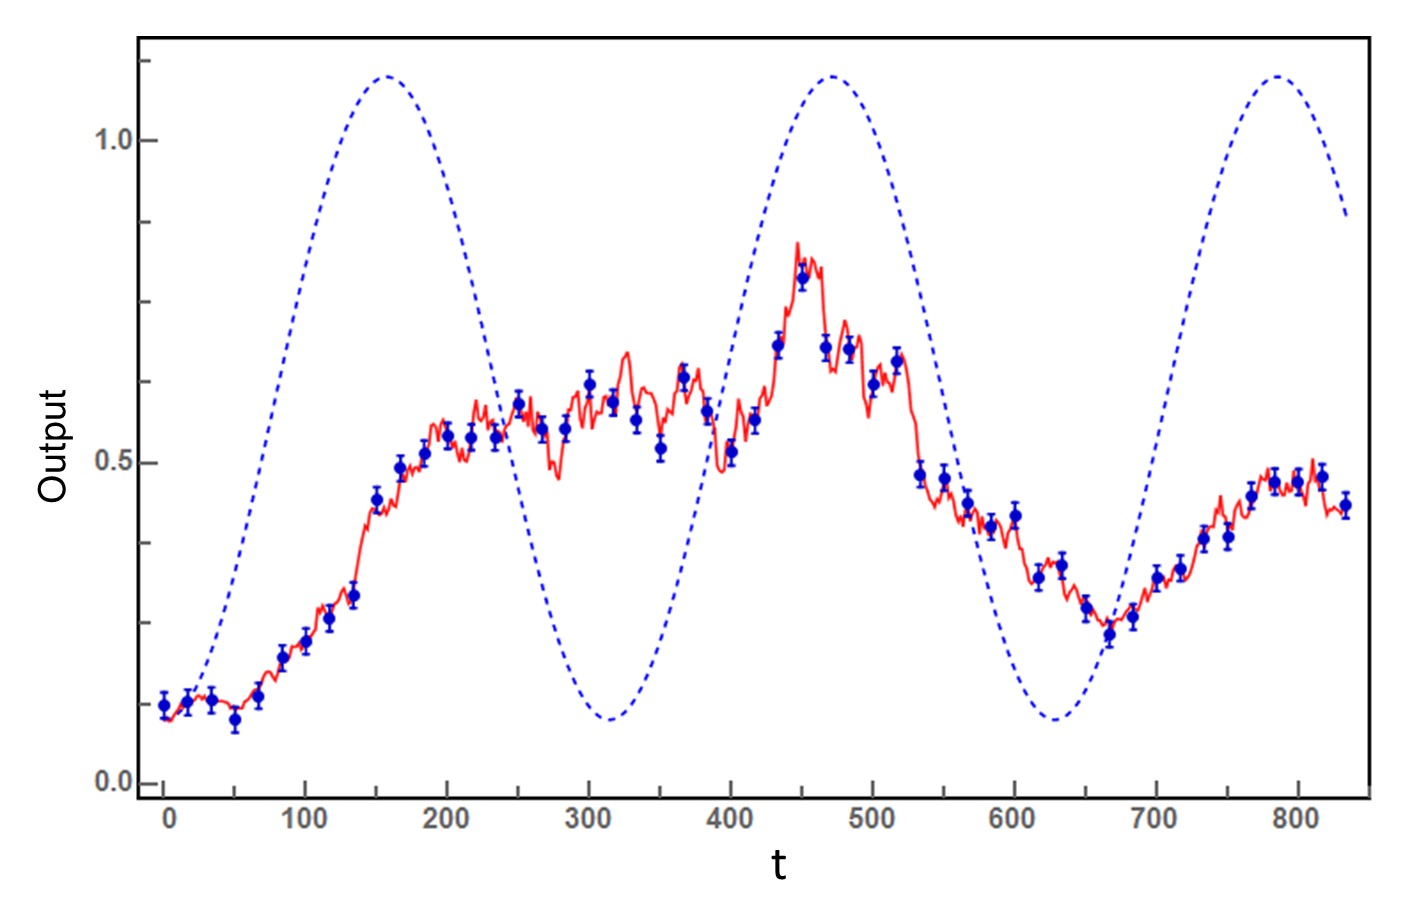
\includegraphics[width=0.7\textwidth]{Figs/FigRainData.png}
    \caption{Rain input (dashed), system realization (solid line) and synthetic experimental data. The system output and the observed data were generated using $K=200$ and $\gamma = 0.2$.}
    \label{fig:rain_data_S}
\end{figure}

\begin{figure}
    \centering
    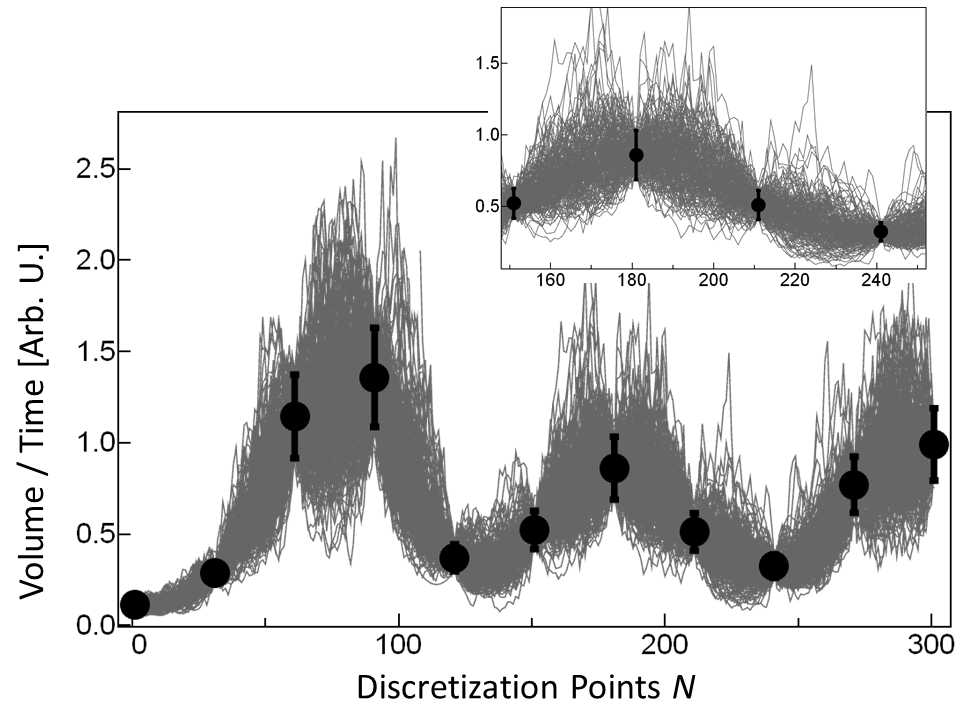
\includegraphics[width=0.9\textwidth]{Figs/FigSpaghetti.png}
    \caption{Simulated system realizations and synthetic experimental data obtained assuming a simple sinusoidal model for the rain input. In the inset one may appreciate the different dynamics of the heavy data-point beads and the light staging beads.}
    \label{fig:spaghetti}
\end{figure}

\begin{figure}
    \centering
    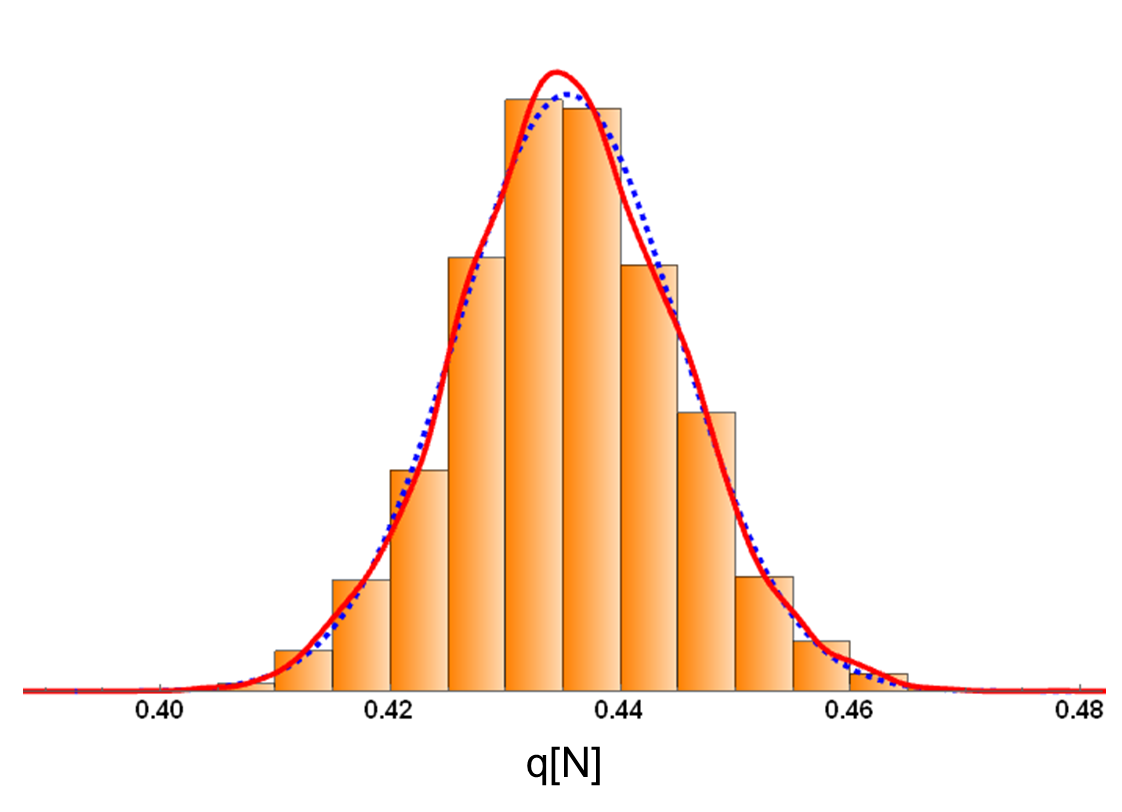
\includegraphics[width=0.6\textwidth]{Figs/FigFinalState.png}
    \caption{PDF for the system final state expressed via the coordinate set $\left\{ q_N \right\}$. The dashed curve represents a normal distribution with the same mean and variance. The final state is basically normally distributed.}
    \label{fig:final_state}
\end{figure}

\begin{figure}
    \centering
    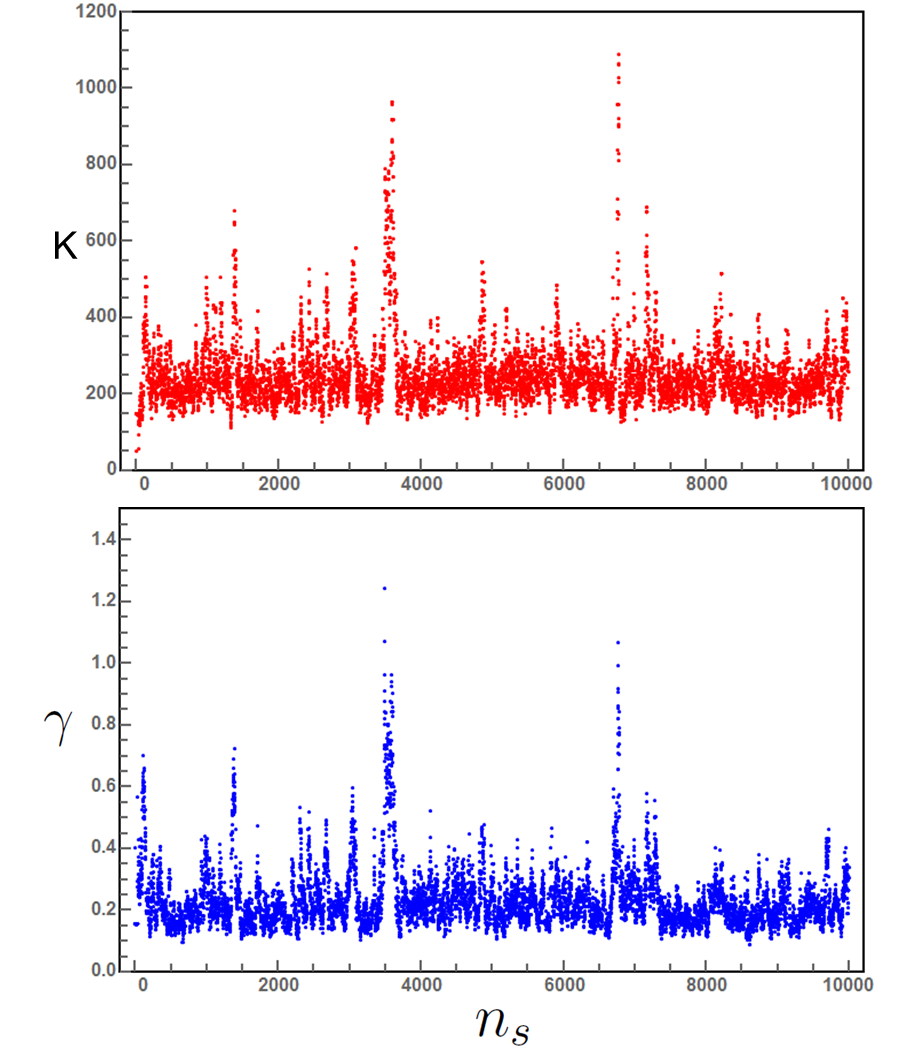
\includegraphics[width=0.7\textwidth]{Figs/FigChains.png}
    \caption{Markov chains for the two parameters $K$ (top) and $\gamma$ (bottom).}
    \label{fig:chains}
\end{figure}

\begin{figure}
    \centering
    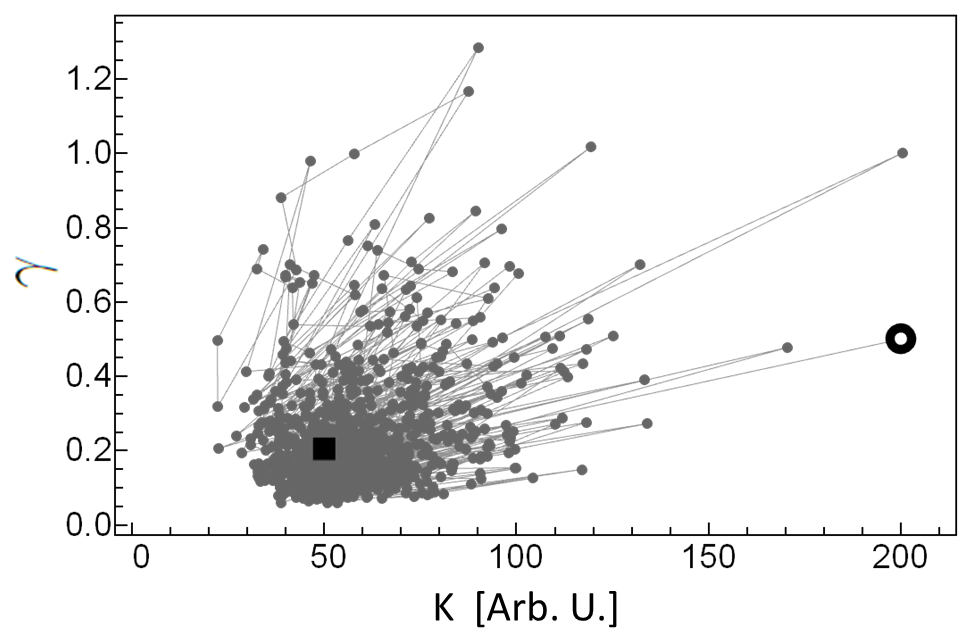
\includegraphics[width=0.9\textwidth]{Figs/FigPhaseSpaceEvol.png}
    \caption{System dynamics in the phase space $K-\gamma$. The green dot is the initial state, the red dot is the final state, the yellow dots are the last 50 states of the HMC chain, and the orange square corresponds to the true parameter values used to generate the data.}
    \label{fig:phase_space_evol}
\end{figure}

\begin{figure}
    \centering
    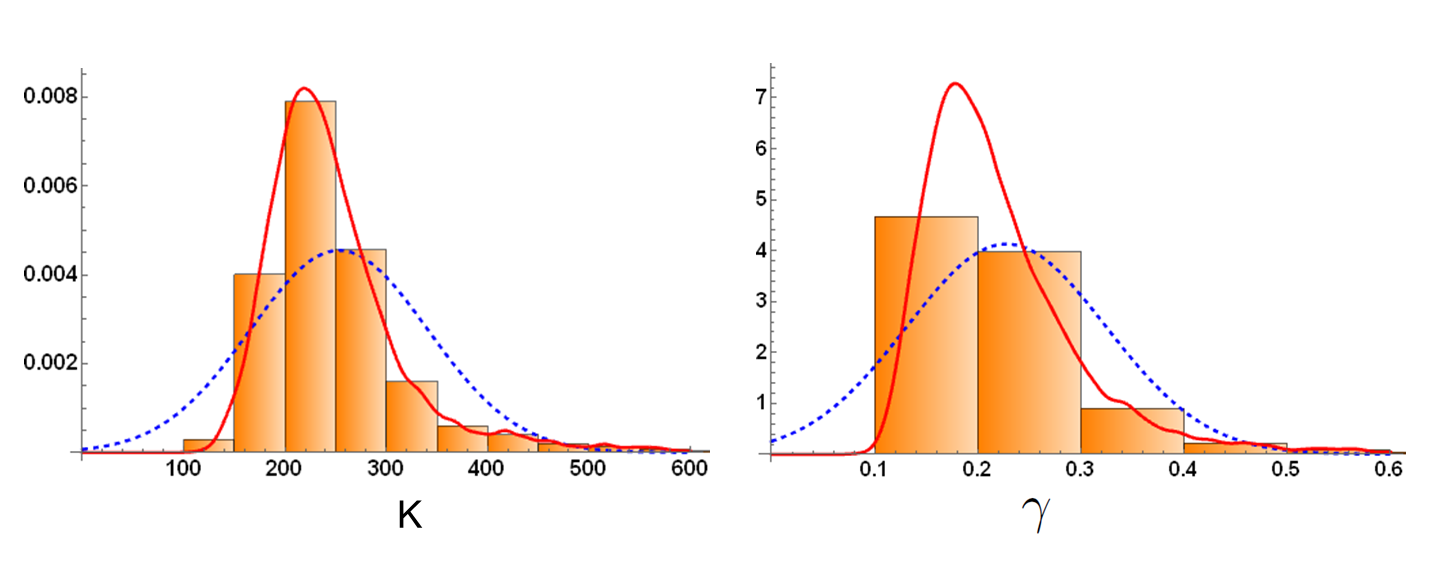
\includegraphics[width=0.9\textwidth]{Figs/FigKg.png}
    \caption{PDF for the parameters $K$ (left) and $\gamma$ (right). The true values used to generate the data are $K=200$ and $\gamma = 0.2$. The initial values used in the simulations were $K=50$ and $\gamma = 0.4$.}
    \label{fig:K_distr}
\end{figure}



\bibliographystyle{apalike} % chicago \shortcite(N)
\bibliography{C:/Users/ulzegasi/SWITCHdrive/refs}



\end{document}
